\documentclass[tikz,border=8pt]{standalone}
\usepackage{tikz}
\usepackage{fontspec}
\setmainfont{DejaVu Sans}
\setsansfont{DejaVu Sans}
\usetikzlibrary{arrows.meta, positioning, shapes.geometric, calc, fit, backgrounds}
\begin{document}
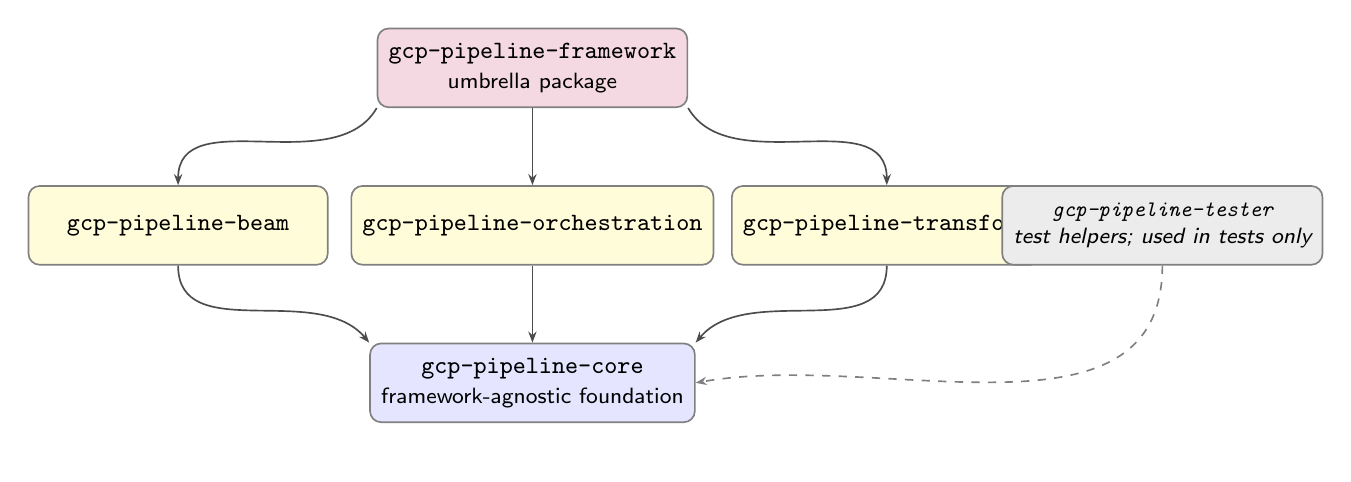
\begin{tikzpicture}[
  font=\sffamily\small,
  every node/.style={font=\sffamily\small},
  box/.style={draw=black!50, line width=0.6pt, rounded corners=4pt, minimum width=2.4cm, minimum height=1cm, align=center, inner sep=4pt},
  src/.style={box, fill=blue!10},
  storage/.style={box, fill=green!10},
  compute/.style={box, fill=yellow!15},
  output/.style={box, fill=purple!15},
  control/.style={box, fill=gray!15, font=\sffamily\footnotesize\itshape},
  err/.style={box, fill=red!10},
  arrow/.style={-{Stealth[length=4pt]}, line width=0.6pt, draw=black!70},
  dashed-arrow/.style={arrow, dashed, draw=black!50},
  caption/.style={font=\sffamily\footnotesize, text=black!60},
  lib/.style={box, minimum width=3.8cm}
]

% Top: umbrella
\node[output, lib] (umbrella) at (4.5, 4)
  {\texttt{gcp-pipeline-framework}\\{\footnotesize umbrella package}};

% Middle three
\node[compute, lib] (beam) at (0, 2)    {\texttt{gcp-pipeline-beam}};
\node[compute, lib] (orch) at (4.5, 2)  {\texttt{gcp-pipeline-orchestration}};
\node[compute, lib] (trans) at (9, 2)   {\texttt{gcp-pipeline-transform}};

% Bottom: core
\node[src, lib] (core) at (4.5, 0)
  {\texttt{gcp-pipeline-core}\\{\footnotesize framework-agnostic foundation}};

% Right side: tester
\node[control, lib] (tester) at (12.5, 2)
  {\texttt{gcp-pipeline-tester}\\{\footnotesize test helpers; used in tests only}};

% Arrows: umbrella -> middle three
\draw[arrow] (umbrella.south west) to[out=-120,in=90] (beam.north);
\draw[arrow] (umbrella.south)      -- (orch.north);
\draw[arrow] (umbrella.south east) to[out=-60,in=90]  (trans.north);

% Arrows: middle three -> core
\draw[arrow] (beam.south)  to[out=-90,in=130] (core.north west);
\draw[arrow] (orch.south)  -- (core.north);
\draw[arrow] (trans.south) to[out=-90,in=50]  (core.north east);

% Dashed arrow: tester -> core
\draw[dashed-arrow] (tester.south) to[out=-90,in=10] (core.east);

\end{tikzpicture}
\end{document}
